\documentclass{article}
\usepackage[utf8]{inputenc}% encodage du fichier source
\usepackage[francais]{babel}% rajouter éventuellement english, greek, etc.
\usepackage{listings}
\usepackage{hyperref}
\usepackage{eurosym}
\usepackage[margin=2.5cm]{geometry}
\usepackage{graphicx}
\hypersetup{urlcolor=,linkcolor=} % Does not apply color to href's
\lstset{
	tabsize=4,
	language=Java,
        basicstyle=\scriptsize,
        columns=fixed,
        extendedchars=true,
        breaklines=true,
		frame=single,
        showtabs=false,
        showspaces=false,
        showstringspaces=false,
        identifierstyle=\ttfamily,
        keywordstyle=\color[rgb]{0,0,1},
        commentstyle=\color[rgb]{0.133,0.545,0.133},
        stringstyle=\color[rgb]{0.627,0.126,0.941},
        numbers=left, 
        numberstyle=\tiny,
        xleftmargin=\parindent
}


\title{ANDROID - TP1}
\date{Source, pdf et corrigé de ce TP
:\\\href{http://tiny.cc/techmob}{http://tiny.cc/techmob}}

\begin{document}
\maketitle
Ce TP a deux objectifs :
\begin{itemize}
\item Se familiariser avec le SDK Android et l'IDE Android Studio
\item Construire une petite application de conversion de devises
\end{itemize}
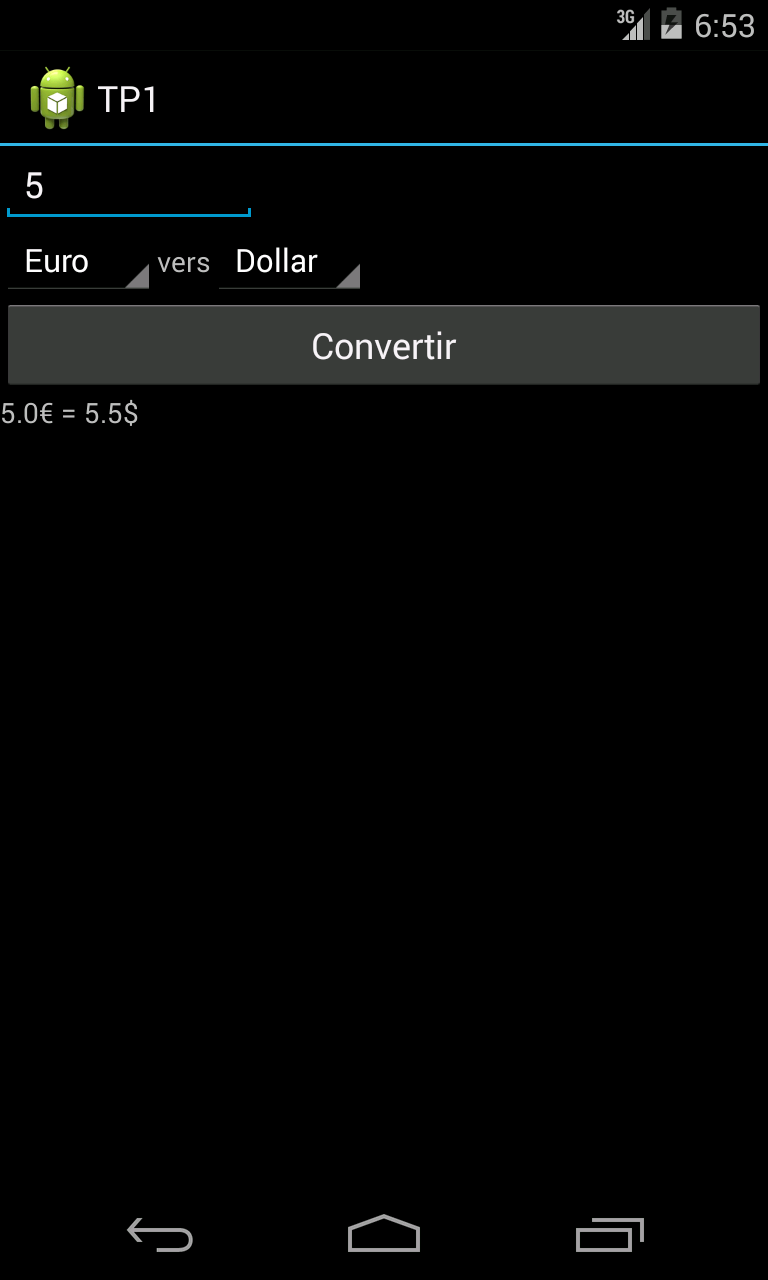
\includegraphics[width=100pt]{img/tp1.png}\\
Il est fortement conseillé d'avoir le cours à portée de main et à ne pas hésiter
à se référer à la documentation officielle
\href{http://d.android.com}{http://d.android.com} ainsi qu'à la multitude de
tutoriaux disponibles.
\section{Mise en place}
\subsection{Verifier l'installation}
\begin{itemize}
\item Lancer Android Studio
\item Vérifier dans \textbf{Tools/Android/SDK Manager} que le chemin vers le SDK
est bien renseigné
\end{itemize}
\begin{enumerate}
\item Quels sont les niveaux d'API disponibles ?
\end{enumerate}
\subsection{Hello world}
\begin{itemize}
\item Créer un nouveau projet android via \textbf{File/New/New Project}
\item On souhaite cibler plus de 95\% des utilisateurs actifs d'Android. Choisir
le bon niveau minimum d'API
\item Notre application ne supportera pour l'instant que les téléphones et les
tablettes
\item Pour simplifier, choisir une Empty Activity
\end{itemize}
Android Studio génère automatiquement toute la structure d'un projet android
gradleisé.
\begin{itemize}
\item Vérifier que la structure générée correspond à la structure vue dans le
cours et que votre projet contient déjà une première activity
\item Lancer l'application
\end{itemize}
\begin{enumerate}
 \setcounter{enumi}{1}
\item Pourquoi l'application ne se lance t'elle pas ?
\end{enumerate}
\begin{itemize}
\item L'Android Virtual Device manager permet de créer un émulateur afin d'y
déployer votre application
\end{itemize}
L'AVD manager est aussi disponible via \textbf{Tools / Android / AVD Manager}
\subsection{Créer un appareil virtuel}
Un émulateur a déjà été crée sur vos postes
\begin{itemize}
\item Vérifier que l'architecture choisie est bien la plus performante pour vos
machines
\item Démarrer l'appareil
\item Manipuler un peu l'émulateur
\item Lancer l'application sur l'émulateur
\end{itemize}
\begin{enumerate}
 \setcounter{enumi}{2}
\item Comment voir la log de l'émulateur ? (2 façons)
\end{enumerate}
\section{Construire notre convertisseur de devises}
\subsection{Logcat}
\begin{itemize}
\item Logger chaque appel à onCreate() en niveau info
\item Verifier dans logcat que les messages apparaissent bien
\end{itemize}
\subsection{Un peu d'IHM}
\begin{itemize}
  \item Simplifier le layout main pour utiliser un LinearLayout
\end{itemize}
Modifier le layout pour y ajouter quelques composants :
\begin{itemize}
\item Un champ de texte modifiable : montant (en euros)
\item Un bouton : convertir
\end{itemize}
\begin{enumerate}
 \setcounter{enumi}{3}
\item Que faut-il prévoir pour pouvoir manipuler ces vues en Java ?
\end{enumerate}
\subsection{Rendre l'interface vivante}
\begin{itemize}
\item Ecouter les clicks sur le bouton et déclencher un toast lors d'un click sur le bouton
\item Dans le toast, afficher le contenu du champ de texte montant
\end{itemize}
Aide : la méthode
\href{http://developer.android.com/reference/android/widget/EditText.html#getText()}{getText()} de EditText permet de récupérer le contenu du champ
\subsection{Implémenter la logique métier}
\begin{itemize}
\item Lors d'un click sur le bouton, récupérer la valeur numérique du montant
\end{itemize}
Aide :
\href{http://developer.android.com/reference/java/lang/Double.html#parseDouble(java.lang.String)}{Double.parseDouble(String)}
permet de convertir une chaîne en nombre à virgule flottante
\begin{itemize}
\item Implémenter la règle métier compliquée suivante : 1\euro  = 1.1\$
\item Afficher le résultat dans un toast
\item Afficher le résultat dans une vue
\end{itemize}
\begin{enumerate}
 \setcounter{enumi}{4}
\item Comment cacher la vue contenant le résultat tant qu'il n'a pas été
calculé ?
\item Que proposez vous si l'utilisateur n'a pas entré de montant ou un montant
invalide ?
\item Que proposez vous pour éviter que l'utilisateur ne rentre un montant
invalide ?
\end{enumerate}
\subsection{Retravailler l'interface}
\begin{itemize}
\item Choisir un ViewGroup simple et adapté pour disposer tous les éléments
\item Mettre le bouton en dessous du champ de texte
\item Modifier les attributs du Button pour lui faire prendre tout l'écran en
largeur
\item Ajouter un attribut ``Hint'' au champ de texte
\end{itemize}
\subsection{En multidevise c'est mieux}
On souhaite maintenant donner le choix à l'utilisateur entre plusieurs
devises.\\
La vue correspondant à un menu déroulant est
\href{http://developer.android.com/guide/topics/ui/controls/spinner.html}{Spinner}.
\begin{itemize}
\item Ajouter deux vues Spinner au layout de l'activity
\end{itemize}
Pour les Spinner basiques, on peut préciser les valeurs possibles en
mettant un string-array dans l'attribut XML ``entries'' de la vue Spinner.
\begin{itemize}
\item Créer, dans strings.xml, un string-array contenant les noms de plusieurs
devises
\item Mettre ce string-array en attribut ``entries'' des Spinner
\item En utilisant la méthode
\href{http://developer.android.com/reference/android/widget/AdapterView.html#getSelectedItemPosition()}{getSelectedItemPosition}, récupérer les langues choisies par l'utilisateur
\item Faire varier le taux de change en fonction des langues choisies
\item En utilisant le fait que des ViewGroup peuvent contenir d'autres
ViewGroup, positionner les spinner sur la même ligne
\end{itemize}
\section{Aller plus loin}
\subsection{Un peu de style}
\begin{itemize}
\item Changer le nom de l'application
\item Changer l'icône de l'application
\end{itemize}
\subsection{Traduire l'application}
\begin{itemize}
\item S'assurer que toutes les strings ont été définies en XML
\item Créer un dossier values-fr et y copier le fichier strings.xml
\item Traduire le contenu de strings.xml
\item Tester sur émulateur en changeant la langue dans le menu
\end{itemize}
\subsection{Partager le résultat}
\begin{itemize}
\item Ajouter un bouton : partager
\item Mettre une icône de partage à ce bouton (setBackgroundResource)
\item Lors d'un click sur le bouton, lancer un intent implicite pour partager le résultat
\end{itemize}
\begin{enumerate}
 \setcounter{enumi}{7}
\item Que se passe-t-il si aucune activity n'est capable de répondre à l'intent
?
\end{enumerate}

\end{document}

